\documentclass[titlepage]{article}
\usepackage{array}
\usepackage{enumerate}
\usepackage{graphicx}
\usepackage{listings}

\begin{document}

\author{Stevan Stanisic and Santana Mach}
\title{COMP 8505 - Final Project \\ Rootkit \\ Design Documents}
\date{Nov 06, 2011}
\maketitle{}

\tableofcontents
\pagebreak

\section{Introduction}

Need an intro...

\section{Program Functionality}

The program will be made up of two executables, a Command and Control Client application and a Backdoor Server application.

The Client should have two modes, of which one will be active at a time:
\begin{itemize}
  \item Command Mode - In which the user can send commands to the Server and optionally receive responses.
  \item Exfiltration Mode - In which the user can update the watch list on the Server.
\end{itemize}

In both modes, the Client will also be listening for Exfiltration transmissions from the server and saving them to disk.

The Server will simultaneously be monitoring its network interfaces for incoming commands from the Client and its list of
watch directories for file changes.

\begin{lstlisting}
Pseudo-code for Client Program
\{
	Pseudo code goes here

	...
\}
\end{lstlisting}

\begin{lstlisting}
Pseudo-code for Server Program
\{
	Pseudo code goes here

	...
\}
\end{lstlisting}

\section{Communication Details}

\subsection{State Machine}

\begin{figure}[htb]                                                                       
  \begin{center}
    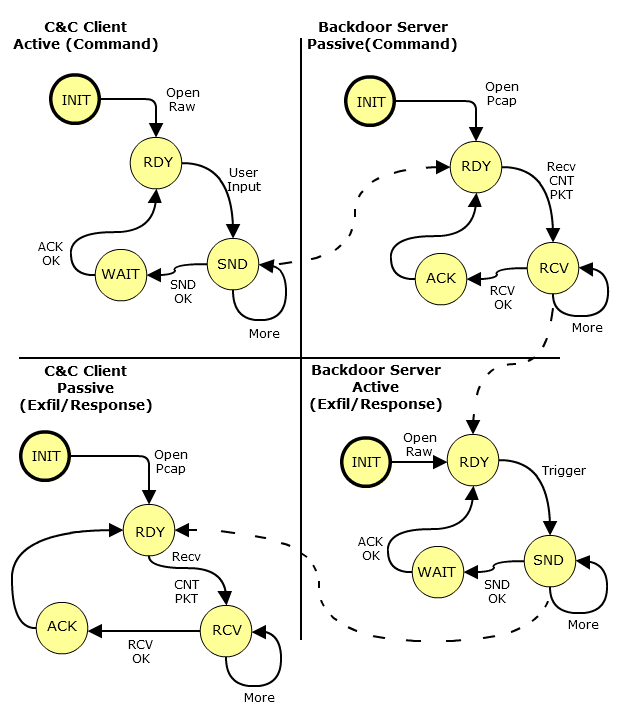
\includegraphics[width=0.9\textwidth]{imgs/std.png}
  \end{center}
  \caption{Program State Transition Diagram}
  \label{fig:std}
\end{figure}

\begin{figure}[htb]                                                                       
  \begin{center}
    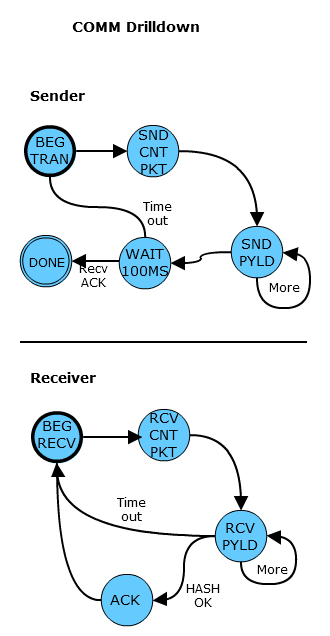
\includegraphics[width=0.5\textwidth]{imgs/comm.png}
  \end{center}
  \caption{Transmission State Transition Diagram}
  \label{fig:comm}
\end{figure}

\begin{lstlisting}
Pseudo-code for State Machine
\{
	Pseudo code goes here

	...
\}
\end{lstlisting}

\subsection{Covert Channel}

\begin{figure}[htb]                                                                       
  \begin{center}
    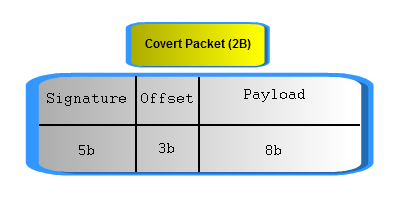
\includegraphics[width=0.9\textwidth]{imgs/packet.png}
  \end{center}
  \caption{Packet Data Diagram}
  \label{fig:packet}
\end{figure}

\begin{figure}[htb]                                                                       
  \begin{center}
    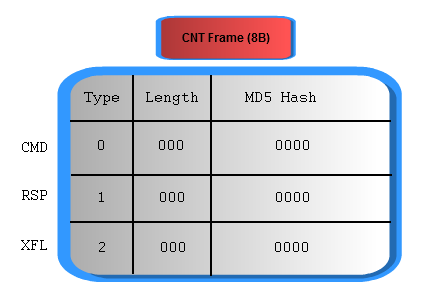
\includegraphics[width=0.9\textwidth]{imgs/frame.png}
  \end{center}
  \caption{Control Frame Diagram}
  \label{fig:frame}
\end{figure}

\begin{figure}[htb]                                                                       
  \begin{center}
    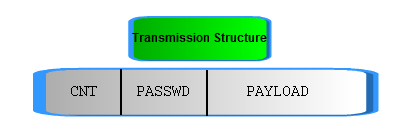
\includegraphics[width=0.9\textwidth]{imgs/transmission.png}
  \end{center}
  \caption{Overall Transmission Diagram}
  \label{fig:transmission}
\end{figure}

\section{Conclusion}

\end{document}
